\documentclass{article}
\usepackage[utf8]{inputenc}
\usepackage{geometry}
% Set the desired page margins
\geometry{
    a4paper,
    left=3cm,
    right=2cm,
    top=3cm,
    bottom=3cm
}
\usepackage[english]{babel}
\usepackage{listings}
\usepackage{booktabs}
\renewcommand{\arraystretch}{1.2}
\usepackage{graphicx}
\usepackage{parskip} 

\setlength{\parindent}{0pt} % Set horizontal indent between paragraphs
\setlength{\parskip}{5pt} % Set vertical spacing between paragraphs

\usepackage{xcolor}
\usepackage{placeins} % Required for \FloatBarrier
\usepackage{float} % Required for H specifier
\usepackage{pgf} % for matplotlib


\usepackage{tikz}
\usetikzlibrary{positioning}

% color def
\usepackage{color}
\definecolor{darkred}{rgb}{0.6,0.0,0.0}
\definecolor{darkgreen}{rgb}{0,0.50,0}
\definecolor{lightblue}{rgb}{0.0,0.42,0.91}
\definecolor{orange}{rgb}{0.99,0.48,0.13}
\definecolor{grass}{rgb}{0.18,0.80,0.18}
\definecolor{pink}{rgb}{0.97,0.15,0.45}

% listings
\usepackage{listings}


\lstdefinelanguage{hist}{
    basicstyle=\fontsize{8}{10}\ttfamily,
}
\definecolor{jsonblue}{RGB}{42,0,255}
\definecolor{jsonpurple}{RGB}{128,0,128}


\lstdefinelanguage{json}{
    basicstyle=\fontsize{8}{10}\ttfamily,
    numbers=left,
    numberstyle=\tiny,
    stepnumber=1,
    numbersep=8pt,
    showstringspaces=false,
    breaklines=true,
    frame=lines,
    backgroundcolor=\color{white},
    literate=
     *{0}{{{\color{jsonpurple}0}}}{1}
      {1}{{{\color{jsonpurple}1}}}{1}
      {2}{{{\color{jsonpurple}2}}}{1}
      {3}{{{\color{jsonpurple}3}}}{1}
      {4}{{{\color{jsonpurple}4}}}{1}
      {5}{{{\color{jsonpurple}5}}}{1}
      {6}{{{\color{jsonpurple}6}}}{1}
      {7}{{{\color{jsonpurple}7}}}{1}
      {8}{{{\color{jsonpurple}8}}}{1}
      {9}{{{\color{jsonpurple}9}}}{1}
      {:}{{{\color{jsonblue}{:}}}}{1}
      {,}{{{\color{jsonblue}{,}}}}{1}
      {\{}{{{\color{jsonblue}{\{}}}}{1}
      {\}}{{{\color{jsonblue}{\}}}}}{1}
      {[}{{{\color{jsonblue}{[}}}}{1}
      {]}{{{\color{jsonblue}{]}}}}{1},
}


% Define custom colors
\definecolor{codegreen}{rgb}{0,0.6,0}
\definecolor{codegray}{rgb}{0.5,0.5,0.5}
\definecolor{codepurple}{rgb}{0.58,0,0.82}

% Define Python style
\lstdefinestyle{mystyle}{
    commentstyle=\color{codegreen},
    keywordstyle=\color{blue},
    numberstyle=\tiny\color{codegray},
    stringstyle=\color{codepurple},
    basicstyle=\ttfamily\footnotesize,
    frame=lines,
    breakatwhitespace=false,         
    breaklines=true,                 
    captionpos=b,                    
    keepspaces=true,                 
    numbers=left,                    
    numbersep=5pt,                  
    showspaces=false,                
    showstringspaces=false,
    showtabs=false,                  
    tabsize=2,
    language=Python
}
\lstset{style=mystyle}

\title{Kilter-Grade-Estimator}
\author{Pascal Lüscher}
\date{}

\begin{document}

\maketitle
\begin{center}
    \includegraphics[width=0.75\textwidth]{./media/KilterBoard.png}    
\end{center}


\section{Data from the Website}

The data from the kilterboard is not accessible to the public. Nonetheless, there exists an official application. Similar to the majority of Android applications, the kilterboard application employs a SQLite database. It is feasible to retrieve the routes from this database provided you possess a rooted mobile device.

Fortunately, an individual has already performed this task and established the website \\https://kilterboard.app. As a result, I crawled this website and gathered approximately 22,000 routes.


\subsection{Data Analysis}

One entry had the following structure

\begin{lstlisting}[language=json, caption={Example of one crawled Entry}]
{
    "uuid": "f01419e1-2672-4593-96ca-62e3655abc46",
    "layout_id": 1,
    "layout_deviant_id": 9,
    "setter_id": 1078,
    "setter_username": "jwebxl",
    "name": "swooped",
    "description": "",
    "hsm": 1,
    "edge_left": 32,
    "edge_right": 88,
    "edge_bottom": 8,
    "edge_top": 152,
    "frames_count": 1,
    "frames_pace": 0,
    "is_draft": false,
    "is_listed": true,
    "created_at": "2018-12-06T21:15:01.127371+00:00",
    "climb_stats": [
        {
            "angle": 0,
            "fa_at": "2019-12-05 16:39:44",
            "climb_uuid": "F01419E12672459396CA62E3655ABC46",
            "fa_username": "sheylo",
            "quality_average": 2.68571,
            "ascensionist_count": 35,
            "difficulty_average": 14.8857
        },
        {
            "angle": 5,
            "fa_at": "2020-06-01 23:37:50",
            "climb_uuid": "F01419E12672459396CA62E3655ABC46",
            "fa_username": "djragan",
            "quality_average": 2,
            "ascensionist_count": 2,
            "difficulty_average": 12
        }
    ],
    "placements": [
        {
            "x": 20,
            "y": 0,
            "type": "FEET-ONLY",
            "ledPosition": 15
        },
        {
            "x": 16,
            "y": 5,
            "type": "START",
            "ledPosition": 244
        },
        {
            "x": 14,
            "y": 35,
            "type": "FINISH",
            "ledPosition": 221
        }
    ],
    "total_ascents": 4778
}
\end{lstlisting}

as you see, there are several ratings per route, depending on the angle. 
There are also properties that should have no impact on the rating, like setter\_username and the creation date.

\pagebreak
\subsubsection{Layouts}
There is the layout\_id and layout\_deviant\_id property. This specifies which Kilterboard is in use.
A quick Histogram shows that the layout 1 is omnypresent and I can drop the others:
\begin{figure}[H]
    \centering
    \includegraphics[width=0.6\textwidth]{../DataAnalysis/histogram_layout_id.pdf}
    \caption{Histogram layout id}\label{fig:histogram_layout_id}
\end{figure}

The same is true for the layout\_deviant\_id. The deviant 9 is omnypresent.

\begin{figure}[H]
    \centering
    \includegraphics[width=0.6\textwidth]{../DataAnalysis/histogram_layout_deviant_id.pdf}
    \caption{Histogram layout deviant id}\label{fig:histogram_layout_deviant_id}
\end{figure}

for completness sake, the two histograms as text

\begin{minipage}{0.45\textwidth}
    \centering
    \lstinputlisting[language=hist]{../DataAnalysis/histogram_layout_id.txt}
\end{minipage}
\hfill
\begin{minipage}{0.45\textwidth}
    \lstinputlisting[language=hist]{../DataAnalysis/histogram_layout_deviant_id.txt}    
\end{minipage}

\subsubsection{Placements}

The placements are the hold itself. The Kilterboard has $35\times36$ Grid.
I first filtered out the outliers that had Y coordinates 36 and higher (it's 0-indexed), there were 61 cases.
I then analyzed the XY-Combinations for the placement. My goal was to create a One-Hot Encoding for every hold on the grid.
Every hold can be classified as foot, hand, starting or finishing hold. 
I then created a one hot encoding for all positions and types (Feet only, Middle, Start and Finish) FO\_1\_0, FO\_1\_1, 1\_2, until S\_35\_35.
Out of the 1225 ($35\cdot35$) positions, there were only 476 in use. 
When considering the possibilities with the type combination ($35\cdot35\cdot4 = 4900$) there were only 1637 combinations used.
As a first step, I go with the relativly sparse matrix.



\subsubsection{Target Variable}
My goal is to predict the difficulty, there is a difficulty average per angle. In a first model, i will use this variable as is.
Maybe I will convert these in categories.


\subsection{DataConversion}

The output model had the following structure:


\begin{lstlisting}[language=json, caption={Example of one crawled Entry}]
    {
        "Uuid":"f01419e1-2672-4593-96ca-62e3655abc46",
        "Angle":0,
        "DifficultyAverage":14.8857,
        "FO_0_0":true,
        "F_0_0":false,
        "M_0_0":false,
        "S_0_0":false,
        "FO_0_1":true,
        "F_0_1":false,
        "M_0_1":false,
        ...
        "S_34_35":false
    }
\end{lstlisting}

\FloatBarrier
\section{Data from the App}
As mentioned previously, the kilterboard app is an app that uses a sqlite database. 
I went ahead and used an online service called genymotion to emulate a rooted android device.
I installed the kilterboard app, connected adb (android debugging bridge) and pulled the database to my local cumputer.
The total cost for this was 0.40 CHF, genymotion is billed by the minute (0.05 CHF per minute)

I found over 200'000 routes in the app database. The app database also gave me further insight in the structure.

The climbs are stored in a table called climbs. Then there is the climbs\_stats table that stores the angels and average difficulties.

\subsection{Placements}
The placements arent stored in a nice way, there is a column in the climbs table called frames with the following structure:

``p1234r12p1238r13\dots'' 

as you can see, the string is divided in pXXXXrYY numbers. 
The p part is the placement id and the r part is the placement role (foot-only, middle, start, finish)

\subsection{Difficulty}

The difficulty conversion is stored in a table called difficulty\_grades

\begin{center}
 \begin{tabular}{@{}r l@{}} \toprule
    Difficulty & Grade \\
    \midrule
    10 & 4a/V0 \\
    11 & 4b/V0 \\
    12 & 4c/V0 \\    
    13 & 5a/V1 \\
    14 & 5b/V1 \\
    15 & 5c/V2 \\
    16 & 6a/V3 \\
    17 & 6a+/V3 \\
    18 & 6b/V4 \\
    19 & 6b+/V4 \\
    20 & 6c/V5 \\
    21 & 6c+/V5 \\
    22 & 7a/V6 \\
    23 & 7a+/V7 \\
    24 & 7b/V8 \\
    25 & 7b+/V8 \\
    26 & 7c/V9 \\
    27 & 7c+/V10 \\
    28 & 8a/V11 \\
    29 & 8a+/V12 \\
    30 & 8b/V13 \\
    31 & 8b+/V14 \\
    \bottomrule
 \end{tabular}
\end{center}

with this information, I decided to go with a categorized approach. The difficulty gap between 5a and 5b is way less than the gap between 7a and 7b.

The distribution seems to be a bit lopsided, the majority of the data begins at 5c and stretches up until around 7b.
\begin{figure}[H]
    \centering    
    \includegraphics[width=0.6\textwidth]{../DataAnalysis/histogram_difficulties.pdf}
    \caption{Histogram difficulties}\label{fig:histogram_difficulties}
\end{figure}

\subsection{DataConversion}

Since the findings from the website data were the same as the ones in the sqlite database, 
I went forward and implemented a program to transform the data in a new sqlite table.

For a first model, i didn't distinguish between the different placement roles. By the way: sqlite has a column limit of 2000 if you ever need to know ;)

 
\begin{table}[ht]
    \begin{center}
    \begin{tabular}{@{}l c c c c r l@{}} 
       \toprule
       uuid & p1447 & p1073 & \ldots & p4845 & angle & difficulty \\
       \midrule
       0062FB249C1645BD98ED3440E8B4669C & 0 & 1 & \ldots & 1 & 45 & 7b/V8 \\
       0070b5e309a2484887a97bc75b7c1bfb & 1 & 0 & \ldots & 0 & 20 & 6b/V4 \\
       \bottomrule
    \end{tabular}
    \end{center}
    \caption{climbs\_cleaned example}\label{tab:climbs_cleaned}
\end{table}

\FloatBarrier\section{Logistic Regression (Base Model)}

\begin{lstlisting}[language=python, caption={Simple logistic regression}]
from sklearn.linear_model import LogisticRegression

logistic_model = LogisticRegression(
    max_iter=2000, 
    n_jobs=16,
    solver='saga',
    verbose=1)  
logistic_model.fit(X_train, y_train)
\end{lstlisting}

This model took around 5 minutes to train. It has an accuracy of 19\%, which sounds pretty bad.

\begin{figure}[H]
    \centering    
    \includegraphics[width=0.8\textwidth]{../Models/LogisticRegression/confusion_matrix.pdf}
    \caption{Confusion matrix logistic regression}\label{fig:conf_logreg}
\end{figure}

A look at the confusion matrix shows that it isn't that bad. The difference between 7a and 7a+.

I trained another model without the + difficulties (6a+ became 6a) and the accuracy became 32\%. 


\begin{figure}[H]
    \centering    
    \includegraphics[width=0.8\textwidth]{../Models/LogisticRegression/confusion_matrix2.pdf}
    \caption{Confusion matrix logistic regression simplified}\label{fig:conf_logreg2}
\end{figure}


\subsection{Evaluation}

This is just a base model. Since the difficulties are close to each others, I will try a regression model, just to double check if this could perform better.

\FloatBarrier\section{Linear Regression}
The first step was to convert the classes back to ordinal values, I simply used an ordinal encoder
\begin{lstlisting}[language=python, caption={Encode categories ordinal}]
    categories = [
        '4a', '4b', '4c', 
        '5a', '5b', '5c', 
        '6a', '6a+', '6b', '6b+', '6c', '6c+', 
        '7a', '7a+', '7b', '7b+', '7c', '7c+', 
        '8a', '8a+', '8b', '8b+', '8c']
    encoder = OrdinalEncoder(categories=[categories])
    y = encoder.fit_transform(y.values.reshape(-1, 1))
\end{lstlisting}

Then I fitted a model and had a look at the results:
\begin{lstlisting}[language=python, caption={Linear regression model}]
    from sklearn.linear_model import LinearRegression

    linear_model = LinearRegression()  
    linear_model.fit(X_train, y_train)
\end{lstlisting}

MAPE: 408364560813897.9

\emph{Learning:} If you have 0 as outputs, MAPE is a very bad measurement, since you have $\infty$ percentage error

I therefore added $1$ to the input and output vector
\begin{itemize}
    \item MAPE: $34\%$
    \item MAE: $2.01$
    \item MSE: $6.71$
\end{itemize}

This doesn't seem too bad, around $\pm2$ grades wrong.
Let's look at the confusion matrix:

\begin{figure}[H]
    \centering    
    \includegraphics[width=0.8\textwidth]{../Models/LinearRegression/confusion_matrix.pdf}
    \caption{Confusion matrix linear regression}\label{fig:conf_linreg}
\end{figure}

The accuracy is 16\%, so it performs worse compared to the logistic regression.

But it wouldn't be fair to compare it without also comparing the simplified version (6a+ $\rightarrow$ 6a)

\begin{itemize}
    \item MAPE: 25\%
    \item MAE: 1.18
    \item MSE: 2.53
    \item Accuracy: 29\% \small{(converted back by rounding and clipping)}
\end{itemize}

\begin{figure}[H]
    \centering    
    \includegraphics[width=0.8\textwidth]{../Models/LinearRegression/confusion_matrix2.pdf}
    \caption{Confusion matrix linear regression simplified}\label{fig:conf_linreg2}
\end{figure}


The accuracy is lower, than the logistic regresison. I will therefore continue to go forward with classifiers instead of regressors.

\section{XGBoost}

XGBoost requires the labels to be in numerical format, therefore I used a LabelEncoder to encode my y values.
Then I fitted an xgboost model:

\begin{lstlisting}[language=python, caption={XGBoost model definition}]
from xgboost import XGBClassifier
clf = XGBClassifier(device='cuda')
clf.fit(X_train, y_train)
\end{lstlisting}

The result, quite underwhelming, an accuracy of 19.7\%. 
\begin{figure}[H]
    \centering    
    \includegraphics[width=0.8\textwidth]{../Models/XGBoost/confusion_matrix.pdf}
    \caption{Confusion matrix XGBoost}\label{fig:conf_xgboost1}
\end{figure}

Since there are several hyper parameters, I performed a gridsearch, which run over 10h on my computer.
The best model performed slightly better
\begin{figure}[H]
    \centering    
    \includegraphics[width=0.8\textwidth]{../Models/XGBoost/confusion_matrix_best_param.pdf}
    \caption{Confusion matrix XGBoost hyperparameter tuned}\label{fig:conf_xgboost1}
\end{figure}
\subsection{Evaluation}
Sadly not that much better\ldots
\section{NN}
Time for the big guns\ldots

and hate tensorflow for not supporting Cuda 12.4..

Therefore let's learn PyTorch (or in modern words: let ChatGPT do it)

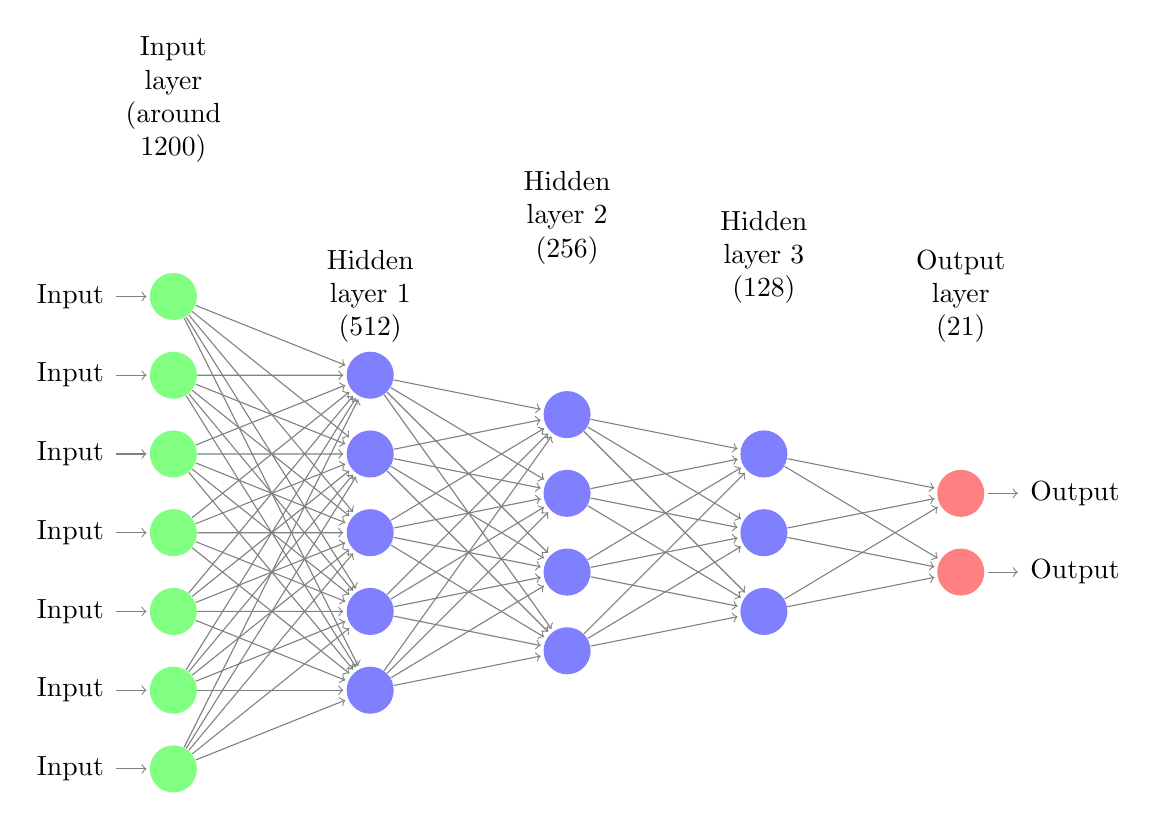
\begin{tikzpicture}[shorten >=1pt,->,draw=black!50, node distance=\layersep]
    \tikzstyle{every pin edge}=[<-,shorten <=1pt]
    \tikzstyle{neuron}=[circle,fill=black!25,minimum size=17pt,inner sep=0pt]
    \tikzstyle{input neuron}=[neuron, fill=green!50];
    \tikzstyle{output neuron}=[neuron, fill=red!50];
    \tikzstyle{hidden neuron}=[neuron, fill=blue!50];
    \tikzstyle{annot} = [text width=4em, text centered]

    \newcommand{\layersep}{2.5cm}

    % Draw the input layer nodes
    \foreach \name / \y in {1,...,7}
        \node[input neuron, pin=left:Input] (I-\name) at (0,-\y cm) {};

    % Draw the hidden layer 1 nodes
    \foreach \name / \y in {1,...,5}
        \path[yshift=-1cm]
            node[hidden neuron] (H1-\name) at (\layersep,-\y cm) {};

    % Draw the hidden layer 2 nodes
    \foreach \name / \y in {1,...,4}
        \path[yshift=-1.5cm]
            node[hidden neuron] (H2-\name) at (2*\layersep,-\y cm) {};

    % Draw the hidden layer 3 nodes
    \foreach \name / \y in {1,...,3}
        \path[yshift=-2cm]
            node[hidden neuron] (H3-\name) at (3*\layersep,-\y cm) {};

    % Draw the output layer nodes
    \foreach \name / \y in {1,...,2}
        \path[yshift=-2.5cm]
            node[output neuron, pin={[pin edge={->}]right:Output}] (O-\name) at (4*\layersep,-\y cm) {};

    % Connect every node in the input layer with every node in the
    % hidden layer 1
    \foreach \source in {1,...,7}
        \foreach \dest in {1,...,5}
            \path (I-\source) edge (H1-\dest);

    % Connect every node in hidden layer 1 with every node in hidden
    % layer 2
    \foreach \source in {1,...,5}
        \foreach \dest in {1,...,4}
            \path (H1-\source) edge (H2-\dest);

    % Connect every node in hidden layer 2 with every node in hidden
    % layer 3
    \foreach \source in {1,...,4}
        \foreach \dest in {1,...,3}
            \path (H2-\source) edge (H3-\dest);

    % Connect every node in hidden layer 3 with every node in output
    % layer
    \foreach \source in {1,...,3}
        \foreach \dest in {1,...,2}
            \path (H3-\source) edge (O-\dest);

    % Annotate the layers
    \node[annot,above of=H1-1, node distance=1cm] (hl1) {Hidden layer 1 (512)};
    \node[annot,above of=H2-1] {Hidden layer 2 (256)};
    \node[annot,above of=H3-1] {Hidden layer 3 (128)};
    \node[annot,above of=I-1] {Input layer (around 1200)};
    \node[annot,above of=O-1] {Output layer (21)};
\end{tikzpicture}

I created a neural network in the most basic architecture, gradually get smaller. 
\subsection{Evaluation}
And the results were stunningly boring again, first the learning curve:

\begin{figure}[H]
    \centering    
    \includegraphics[width=0.8\textwidth]{../Models/NN/nn_learning_curve_epoch_50.pdf}
    \caption{Learning curve of NN}\label{fig:learning_curve_nn}
\end{figure}

As you can see, the loss doesn't really get better after a few epochs.
And the accuracy is still in the 20s.
At this point I think a regression solver might work better. Let's try a NN as a regression solver:

\section{NN Regression}


\input{nn_regressor.tex}

Let's start simple and reuse the classifier NN and just exchange the output layer to be a single node. and train it for 100 epochs:
\begin{figure}[H]
    \centering    
    \includegraphics[width=0.8\textwidth]{../Models/NN_Linear/nn_learning_curve_epoch_100.pdf}
    \caption{Learning curve of NN after 100 epochs}\label{fig:learning_curve_nn_linear_100}
\end{figure}
well that looks like I need some more training time, still the results after 100 epochs are ok:

\begin{itemize}
    \item MSE: 3.5249
    \item MAE: 1.4194
    \item MAPE: 0.2341
\end{itemize}

The absolute error shows that it's $\pm 1.41$ grade. In my context this means a 6a could be a 6a+ or a 5c.
I think this is pretty good (as a comparison: the baseline linear regression was MAE 2.01)

The longer trained model yielded similar results:
\begin{figure}[H]
    \centering    
    \includegraphics[width=0.8\textwidth]{../Models/NN_Linear/nn_learning_curve_epoch_251.pdf}
    \caption{Learning curve of NN after 250 epochs}\label{fig:learning_curve_nn_linear_250}
\end{figure}

\begin{itemize}
    \item MSE: 3.5030
    \item MAE: 1.4117
    \item MAPE: 0.2320
\end{itemize}


\section{Better quality  Train Dataset}
Maybe the models perform not so good because there are a lot of routes that are only climbed by one climber.
And this climber sets the grade, so there is no cross-validation. 

The distribution graph shows that this is indeed the case for many routes:

\begin{figure}[H]
    \centering    
    \includegraphics[width=0.8\textwidth]{../DataAnalysis/ascensionist_count.pdf}
    \caption{Ascensionist Count}\label{fig:asc_count}
\end{figure}

I decided to train a model with only routes that have at least 3 ascensionist.
By doin this I reduce the dataset size from around $173'000$ to $51'000$

\section{NN quality-data}

First again the learning curve
\begin{figure}[H]
    \centering    
    \includegraphics[width=0.8\textwidth]{../Models/NN_reduced_linear/nn_learning_curve_epoch_251.pdf}
    \caption{Learning curve of NN}\label{fig:learning_curve_nn}
\end{figure}
After a bit more than 100 epochs, the learning curve converges.
let's have a look at the results:

\begin{itemize}
    \item MSE: 2.9150
    \item MAE: 1.2868
    \item MAPE: 0.2250
\end{itemize}

I'm now satisfied with the results, a MAE of 1.28 is quite good!

Still I'll train a model with simplified classes ($6a+ \rightarrow 6a$)

Look at these results:

\begin{figure}[H]
    \centering    
    \includegraphics[width=0.8\textwidth]{../Models/NN_reduced_linear/confusion_matrix_simplified.pdf}
    \caption{Confusion matrix NN simplified}\label{fig:conf_nn_red_simpl}
\end{figure}

They look pretty good, some metrics :
\begin{itemize}
    \item MSE: 1.2149
    \item MAE: 0.8097
    \item MAPE: 0.1740
\end{itemize}



\end{document}
